\ylDisplay{Valgustamine} % Ülesande nimi
{Valter Kiisk} % Autor
{lõppvoor} % Voor
{2015} % Aasta
{G 2} % Ülesande nr.
{3} % Raskustase
{
% Teema: Geomeetriline-optika
\ifStatement
Lääts fookuskaugusega $f_1=\SI{4}{cm}$ on paigutatud nii, et läätsele suunatud paralleelsete valguskiirte kimp diameetriga $d_0=\SI{1}{cm}$ koondub ekraanil ühte punkti. Mõnikord on tarvis valgustada ekraanil suuremat ala, kuid läätse nihutamine või valgusallika vahetamine pole võimalik. Kui suur peab olema olemasolevast läätsest paremale paigutatava lisaläätse fookuskaugus $f_2$, et ekraanil tekiks ühtlaselt valgustatud laik diameetriga $d=\SI{2}{cm}$, kui läätsede vahekaugus on $L$?
\begin{center}
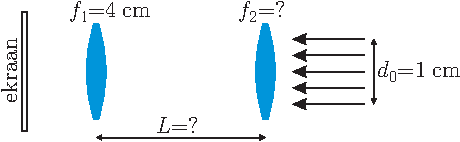
\includegraphics[scale=1.5]{2015-v3g-02-valgustamine-yles}
\end{center}
\fi


\ifHint
Antud juhul tasub vaadelda kõige äärmisi süsteemi sisenevaid kiiri.
\fi


\ifSolution
Vaatleme kõige äärmiste valguskiirte liikumist läbi süsteemi. 
\begin{center}
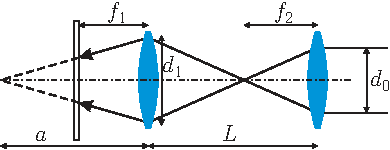
\includegraphics[scale=1.5]{2015-v3g-02-valgustamine-lah}
\end{center}
Pärast lisaläätse läbimist koonduvad valguskiired punktiks lisaläätsest kaugusel $f_2$ ehk kaugusel $L-f_2$ algsest läätsest. Läätse valemi 
\begin{equation}
\frac{1}{a}+\frac{1}{L-f_2}=\frac{1}{f_1}.
\end{equation}
põhjal tekib sellest punktist omakorda punktkujutis kaugusele $a$ esimesest läätsest. Sarnastest kolmnurkadest saame veel kaks võrrandit:
\begin{equation}
\frac{d_1}{d_0}=\frac{L-f_2}{f_2},
\end{equation}
\begin{equation}
\frac{d}{a-f_1}=\frac{d_1}{a}.
\end{equation}
Kahest esimesest võrrandist saame suuruse $\frac{1}{L-f_2}$ avaldamisel
\begin{equation}
\frac{1}{a}+\frac{d_0}{d_1f_2}=\frac{1}{f_1}\implies \frac{d_0}{d_1f_2}=\frac{a-f_1}{af_1}.
\end{equation}
Viimasest kahest võrrandist saame avaldada suuruse $d_1(a-f_1)/a$, mille põhjal saame $d=d_0\frac{f_1}{f_2}.$ Seega valguslaigu suurus ekraanil sõltub ainult lisatud läätse fookuskaugusest, aga mitte läätsedevahelisest kaugusest $L$. Valguslaik diameetriga \SI{2}{cm} tekib kui $f_2=f_1d_0/d=\SI{2}{cm}$.
\fi


\ifEngStatement
% Problem name: Lighting
A lens with a focal length $f_1=\SI{4}{cm}$ is positioned so that a parallel light beam of diameter $d_0=\SI{1}{cm}$ is focused at one point on the screen. Sometimes a bigger area is needed to be lighted on the screen but moving the lens or changing the source of the light is impossible. How big has to be the focal length $f_2$ of an additional lens positioned to the right of the initial lens, so that an evenly lighted area with a diameter $d=\SI{2}{cm}$ would appear on the screen? The distance between the lenses is $L$.
\begin{center}
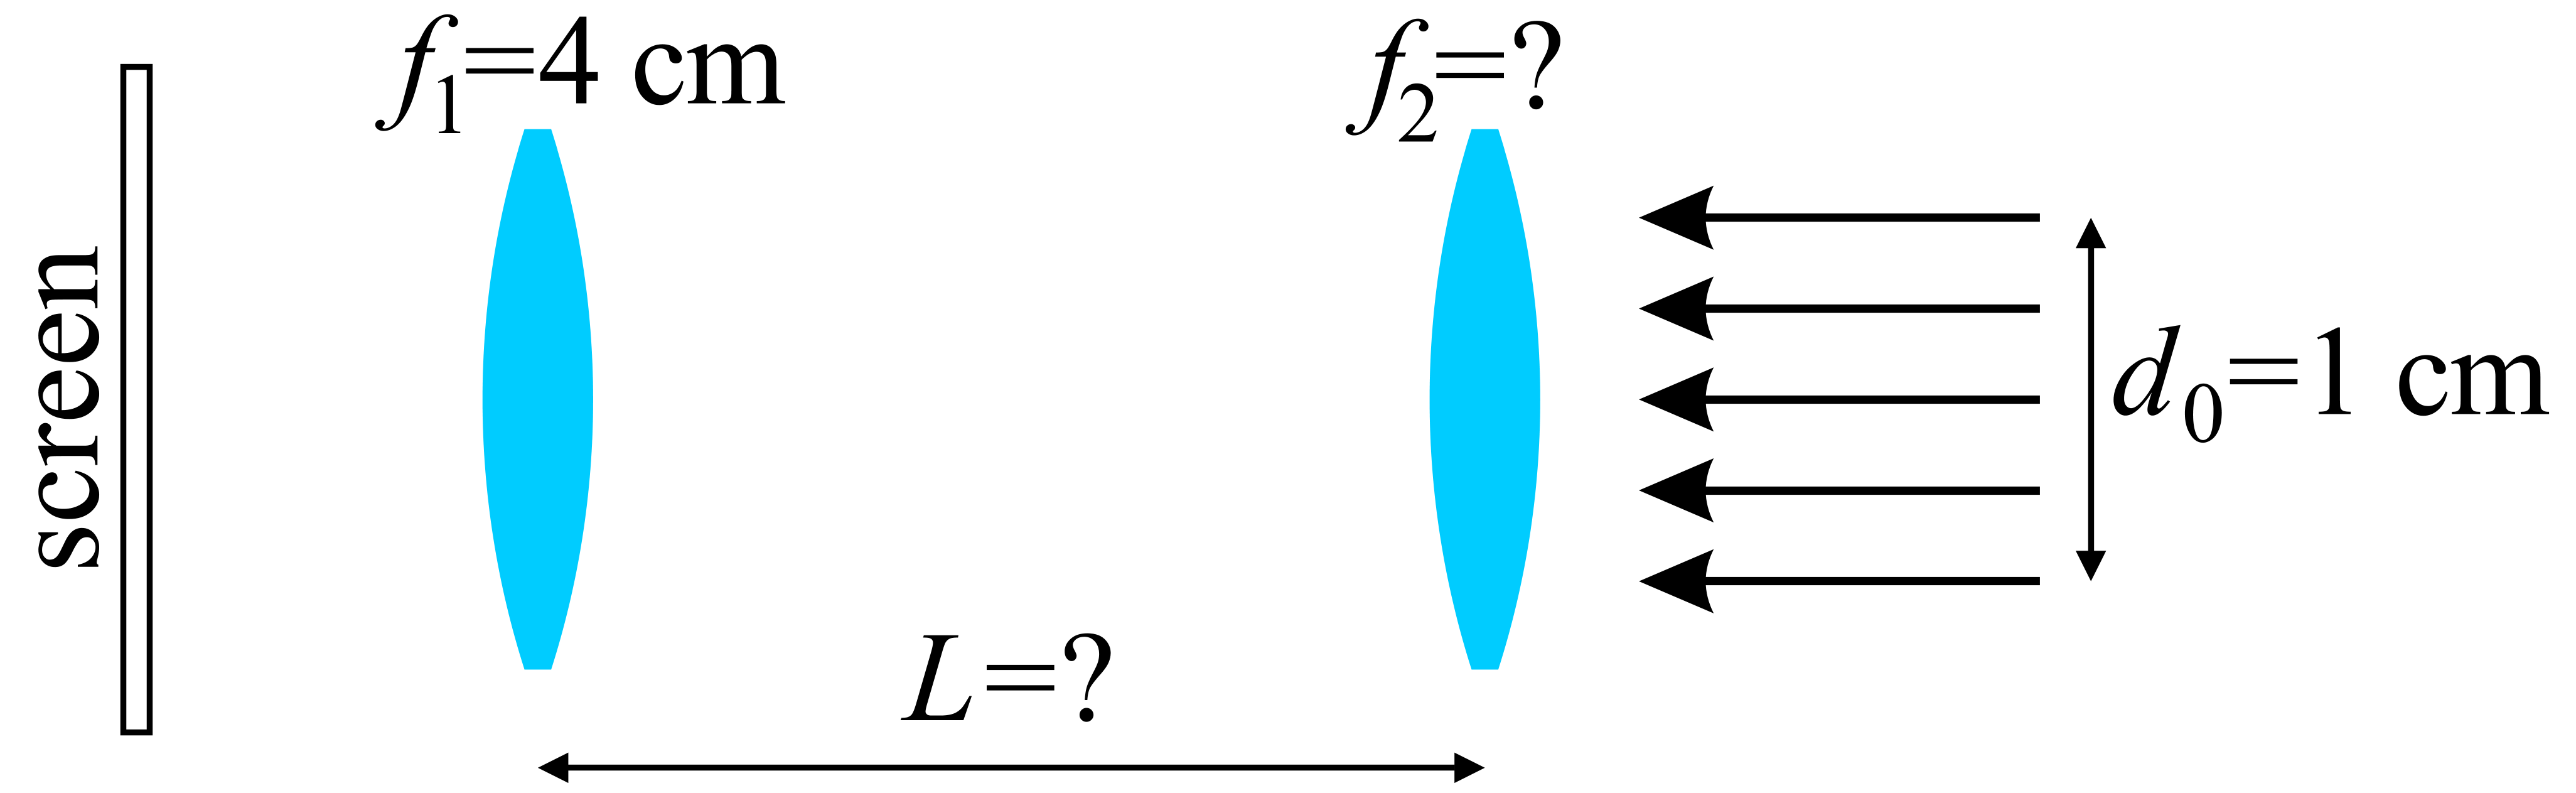
\includegraphics[scale=1.5]{2015-v3g-02-valgustamine-yles_ing}
\end{center}
\fi


\ifEngHint
In the given situation you should observe the outermost rays entering the system.
\fi


\ifEngSolution
Let us observe the paths of the outermost rays through the system.
\begin{center}
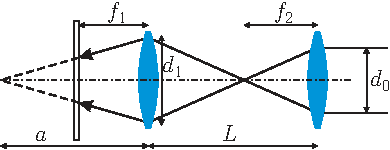
\includegraphics[scale=1.5]{2015-v3g-02-valgustamine-lah}
\end{center}
After going through the additional lens the rays focus to a point at a distance $f_2$ from the additional lens, meaning at a distance $L-f_2$ from the initial lens. Based on the thin lens formula
\begin{equation}
\frac{1}{a}+\frac{1}{L-f_2}=\frac{1}{f_1}.
\end{equation} 
a point image of this point forms in turn at a distance $a$ from the first lens. From similar triangles we get another two equations:
\begin{equation}
\frac{d_1}{d_0}=\frac{L-f_2}{f_2},
\end{equation} 
\begin{equation}
\frac{d}{a-f_1}=\frac{d_1}{a}.
\end{equation}
Expressing the value $\frac{1}{L-f_2}$ from the first two equations we get
\begin{equation}
\frac{1}{a}+\frac{d_0}{d_1f_2}=\frac{1}{f_1}\implies \frac{d_0}{d_1f_2}=\frac{a-f_1}{af_1}.
\end{equation} 
We can express the value $d_1(a-f_1)/a$ from the last two equations and based on this we get $d=d_0\frac{f_1}{f_2}.$. Therefore the size of the lighted area only depends on the focal length of the additional lens but not on the distance $L$ between the lenses. A lighted area of diameter 2 cm appears if $f_2=f_1d_0/d=\SI{2}{cm}$.
\fi
}